%&../settings/preamble.main

\ifsubfile
\appendix
\pagestyle{plain}

% arara: pdflatex: { options: ["--output-directory=../build/chapters"], draft: yes, synctex: no }
% arara: pdflatex: { options: ["--output-directory=../build/chapters"], synctex: no }
\begin{document}
\fi
\chapter{Algoritmi di ordinamento}

\section*{Introduzione}

Durante il corso abbiamo visto alcuni algoritmi di ordinamento, le loro complessità sono riassunte nella tabella~\ref{tab:sorting-complexity}.

\begin{table}[H]\centering
    \caption{Complessità degli algoritmi di ordinamento}
    \label{tab:sorting-complexity}
    \begin{tabular}{@{} l cc l @{}}
    \toprule
        \textbf{Algoritmo} & \textbf{Caso ottimo} & \textbf{Caso pessimo} & \textbf{Tecnica utilizzata}\\
    \midrule
        SelectionSort & \(\Omega(n)\) & \(\Omicron(n)\) & \multicolumn{1}{c}{-}\\
    \lightrule
        InsertionSort & \(\Omega(n)\) & \(\Omicron(n^2)\) & \multicolumn{1}{c}{-}\\
    \lightrule
        ShellSort & \(\Omega(n)\) & \(\Omicron(n^{3/2})\) & ricerca locale\\
    \lightrule
        MergeSort & \multicolumn{2}{c}{\(\Theta(n \log n)\)} & dividi-et-impera\\
    \lightrule
        HeapSort & \multicolumn{2}{c}{\(\Theta(n \log n)\)} & \multicolumn{1}{c}{-}\\
    \lightrule
        QuickSort & \(\Omega(n \log n)\) & \(\Omicron(n^2)\) & \multicolumn{1}{c}{-}\\
    \bottomrule
    \end{tabular}
\end{table}

\shellSort ha una complessità \enquote{migliore} di \insertionSort \(n^{3/2} = n \sqrt{n})\).
Sappiamo inoltre che \quickSort nel caso medio ha una complessità di \(n \log n\).

Possiamo arrivare alla conclusione che tutti questi algoritmi sono \emph{basati su confronti}: le decisioni sull'ordinamento vengono prese in base al confronto (\(<\), \(=\), \(>\)) fra due valori.
Esistono altri modi per ordinare gli oggetti, ma gli algoritmi generali devono essere necessariamente basati sui confronti.

Gli algoritmi migliori che abbiamo visto finora hanno una complessità di \(\Omicron(n \log n)\), \insertionSort e \shellSort sono più veloci (\(\Omega(n)\) solo in casi speciali, è quindi lecito chiederci se sia possibile fare meglio di così.

\section*{Dimostrazione del limite inferiore del problema dell'ordinamento}

\`E possibile dimostrare che qualunque algoritmo di ordinamento \emph{basato sui confronti} ha una complessità di \(\Omega(n \log n)\).

Partiamo facendo alcune assunzioni.
Consideriamo un qualunque algoritmo basato su confronti.
Assumiamo che tutti i valori siano distinti (non abbiamo perdita di generalità).
L'algoritmo può essere quindi rappresentato tramite un \emph{albero di decisione}, ossia un albero binario che rappresenta i confronti con gli elementi.

% \begin{figure}[H]\centering
%     \documentclass[varwidth, tikz]{standalone}
\usepackage{../tikz-preamble}
\usepackage{../../../libraries/set-forest}

% arara: pdflatex: { draft: yes }
% arara: pdflatex: { synctex: no }
% arara: latexmk:  { clean: partial }
\begin{document}
\begin{forest}
    math tree,
    for tree = {
        rounded corners
    },
    % tex.stackexchange.com/questions/280331/
    before typesetting nodes = {
        where n children = 0 {
                draw, fit=band, rounded corners, math content, blue,
                append = {
                    [, draw, rounded corners, fit=band, math content, gray, tier = terminal, edge = dotted, content/.pgfmath = content("!u")]
                }
        }{}
    }
    [1:2
        [2:3, edge label={node[midway, above left]{\(<\)}}
            [{1,2,3}, edge label={node[midway, above left]{\(<\)}}]
            [1:3, edge label={node[midway, above right]{\(>\)}}
                [{1,3,2}, edge label={node[midway, left]{\(<\)}}]
                [{3,1,2}, edge label={node[midway, right]{\(>\)}}]
            ]
        ]
        [1:3, edge label={node[midway, above right]{\(>\)}}
            [{2,1,3}, edge label={node[midway, above left]{\(<\)}}]
            [2:3, edge label={node[midway, above right]{\(>\)}}
                [{2,3,1}, edge label={node[midway, left]{\(<\)}}]
                [{3,2,1}, edge label={node[midway, right]{\(>\)}}]
            ]
        ]
    ]
\end{forest}
\end{document}

%     \caption{Albero di decisione}
% \end{figure}

Gli alberi di decisione hanno due proprietà:
\begin{enumerate}
    \item il \emph{cammino radice-foglia} rappresenta la sequenza di confronti eseguiti dall'algoritmo corrispondente;
    \item l'\emph{altezza dell'albero} rappresenta il numero di confronti eseguiti dall'algoritmo corrispondente nel caso pessimo.
\end{enumerate}

Si considerino tutti gli alberi di decisione ottenibili da algoritmi di ordinamento basati su confronti.

\begin{lemma}
Un albero di decisione per l'ordinamento di \(n\) elementi contiene \textbf{almeno} \(n!\) foglie.
\end{lemma}

Questo accade perché le foglie rappresentano il modo in cui dobbiamo scambiare i valori e siccome \(n!\) è una qualsiasi delle permutazioni in cui riceviamo il nostro input, l'albero di decisione corrispondente deve avere una foglia per ogni suo elemento.
Potrebbe averne anche più di una foglia, in quanto l'algoritmo potrebbe non essere efficiente ed effettuare più ordinamenti di quanto ne siano necessari, ma deve averne \emph{almeno} \(n!\).

Ora possiamo restringerci al caso dell'albero binario in quanto abbiamo valori distinti e lo possiamo fare senza perdere generalità.

\begin{lemma}
Sia \(T\) un albero binario in cui ogni nodo interno ha esattamente \(2\) figli (\(<\) e \(>\)) e sia \(k\) il numero delle sue foglie.
Allora l'altezza dell'albero è \textbf{almeno} \(\log k\) ovvero \(\Omega(n \log n)\).
\end{lemma}

L'altezza sarà \(\log k\) solo se l'albero è perfettamente bilanciato.

\begin{theorem}
Il numero di confronti necessari per ordinare \(n\) elementi nel caso peggiore è \(\Omega(n \log n)\).
\end{theorem}

Abbiamo \(n!\) foglie, quindi l'altezza dell'albero è \(\sim \log n!\) e abbiamo che \(\sim n \log n\).

\section{Algortimi non basati sui confronti}

\subsection{Spaghetti Sort}

L'algoritmo \spaghettiSort è caratterizzato da 5 fasi:
\begin{enumerate}
    \item prendi \(n\) spaghetti;
    \item taglia lo spaghetto \(i\)-esimo in modo proporzionale all'\(i\)-esimo valore da ordinare;
    \item con la mano, afferra gli \(n\) spaghetti e appoggiali verticalmente sul tavolo;
    \item prendi il più lungo, misuralo e metti il valore corrispondente in fondo al vettore da ordinare;
    \item ripeti il passo 4 fino a quando non hai terminato gli spaghetti.
\end{enumerate}

Nel modo in cui è stato descritto questo algoritmo è infinitamente parallelo: qualsiasi sia il numero di spaghetti potremmo trovare lo spaghetto più lungo in \(\Omicron(1)\).
Quindi questo algoritmo ha una complessità di \(\Omicron(n)\).

\subsection{Counting Sort}

Assumiamo che i numeri da ordinare siano compresi in un intervallo \([1 \dots k]\) (questo algoritmo non funziona con le stringhe).

\paragraph{Come funziona}
Costruisce un vettore di appoggio \(B[1 \dots k]\) che conta il numero di volte che un valore compreso in \([1 \dots k]\) compare in \(A\).
Ricolloca i valori così ottenuti nel vettore da ordinare \(A\).

\begin{note}
L'intervallo non deve necessariamente iniziare in \(1\) e finire in \(k\); qualunque intervallo di cui conosciamo gli estremi può essere utilizzato nel Counting Sort.
\end{note}

\begin{algorithm}[H]
    \caption{Algoritmo di ordinamento Counting Sort}
    %&../preamble

% arara: pdflatex: { synctex: no }
% arara: latexmk: { clean: partial }
\ifstandalone
\begin{document}
\begin{algorithm}[H]
\fi
\prototype{\countingSort{\Item{} A, \Int n, \Int k}}{

	\BlankLine
	% \Int i, j, k\;
	\Array{\Int} \(B\) \Assign \new \Array{\Int}[1][k] \tcp{creo il vettore d'appoggio}

	\BlankLine
	% \tcp{Inizializza i vettori}
	\For(\tcp*[h]{\(\Omicron(k)\)}){\(i \Assign 1\) \DownTo \(k\)}{
		\(B[i] = 0\) \tcp{azzero il vettore d'appoggio}
	}

	\BlankLine
	\For(\tcp*[h]{\(\Omicron(n)\)}){\(j \Assign 1\) \DownTo \(n\)}{
		\(B[A[j]] = B[A[j]] + 1\) \tcp{conto quante volte incontro quel valore}
	}

	\BlankLine
	\tcp{vado a ricollocare i vari valori man mano che li incontro}
	\(j = 1\) \tcp{partendo dalla prima posizione}
	\From(\tcp*[h]{scorro tutto il vettore}){\(i=1\) \DownTo \(k\)}{
		\While(\tcp*[h]{per tutte le occorrenze di un determinato valore}){\(B[i] > 0\)}{
			\(A[j] \Assign i\) \tcp{lo inserisco nel vettore}
			\(\Increment{j}\) \tcp{scorro il cursore}
			\(B[i] \Assign B[i] - 1\) \tcp{diminuisco le occorrenze}
		}
	}
}
\ifstandalone
\end{algorithm}
\end{document}
\fi

\end{algorithm}

\paragraph{Complessità}
Inizializzare il vettore d'appoggio costa \(\Omicron(k)\).
Contare le occorrenze di un valore costa \(\Omicron(n)\), in quanto fare riferimento ad una casella di memoria dato un valore costa \(\Omicron(1)\) e lo faccio \(n\) volte.
L'algoritmo ha una complessità totale di \(\Omicron(n+k)\).
Se \(k\) è \(\Omicron(n)\), allora la sua complessità è \(\Omicron(n)\).

Questo algoritmo non è basato sui confronti.
Abbiamo quindi cambiato le condizioni di base e la dimostrazione che abbiamo visto per il limite inferiore non vale.
Ad esempio se \(k\) è \(\Omicron(n^3)\) questo algoritmo è peggiore di tutti quelli visti finora.

\clearpage
\subsection{Pigeonhole Sort}

Se dobbiamo ordinare chiavi numeriche basse e valori associati, allora possiamo usare \pigeonholeSort.
Sfruttiamo lo stesso meccanismo di \countingSort, ma anziché contare le occorrenze le inseriamo all'interno di una lista concatenata.
L'inserimento di un elemento in una lista ha costo \(\Omicron(1)\), quindi l'algoritmo ha \(\Omicron(n)\) a patto che sia possibile limitare l'input a \(k\) elementi (possibilmente piccolo).
Il costo complessivo risulta quindi \(\Omicron(n+k)\) e vale considerazione precedente.so

\begin{note}
\pigeonholeSort è un'estensione del \countingSort che permette di ordinare in tempo lineare coppie (chiave, valore), invece che singoli interi.
Le chiavi devono essere comprese fra \(1\) e \(k\) (con \(k\) possibilmente piccolo).
\end{note}

\begin{figure}[H]\centering
    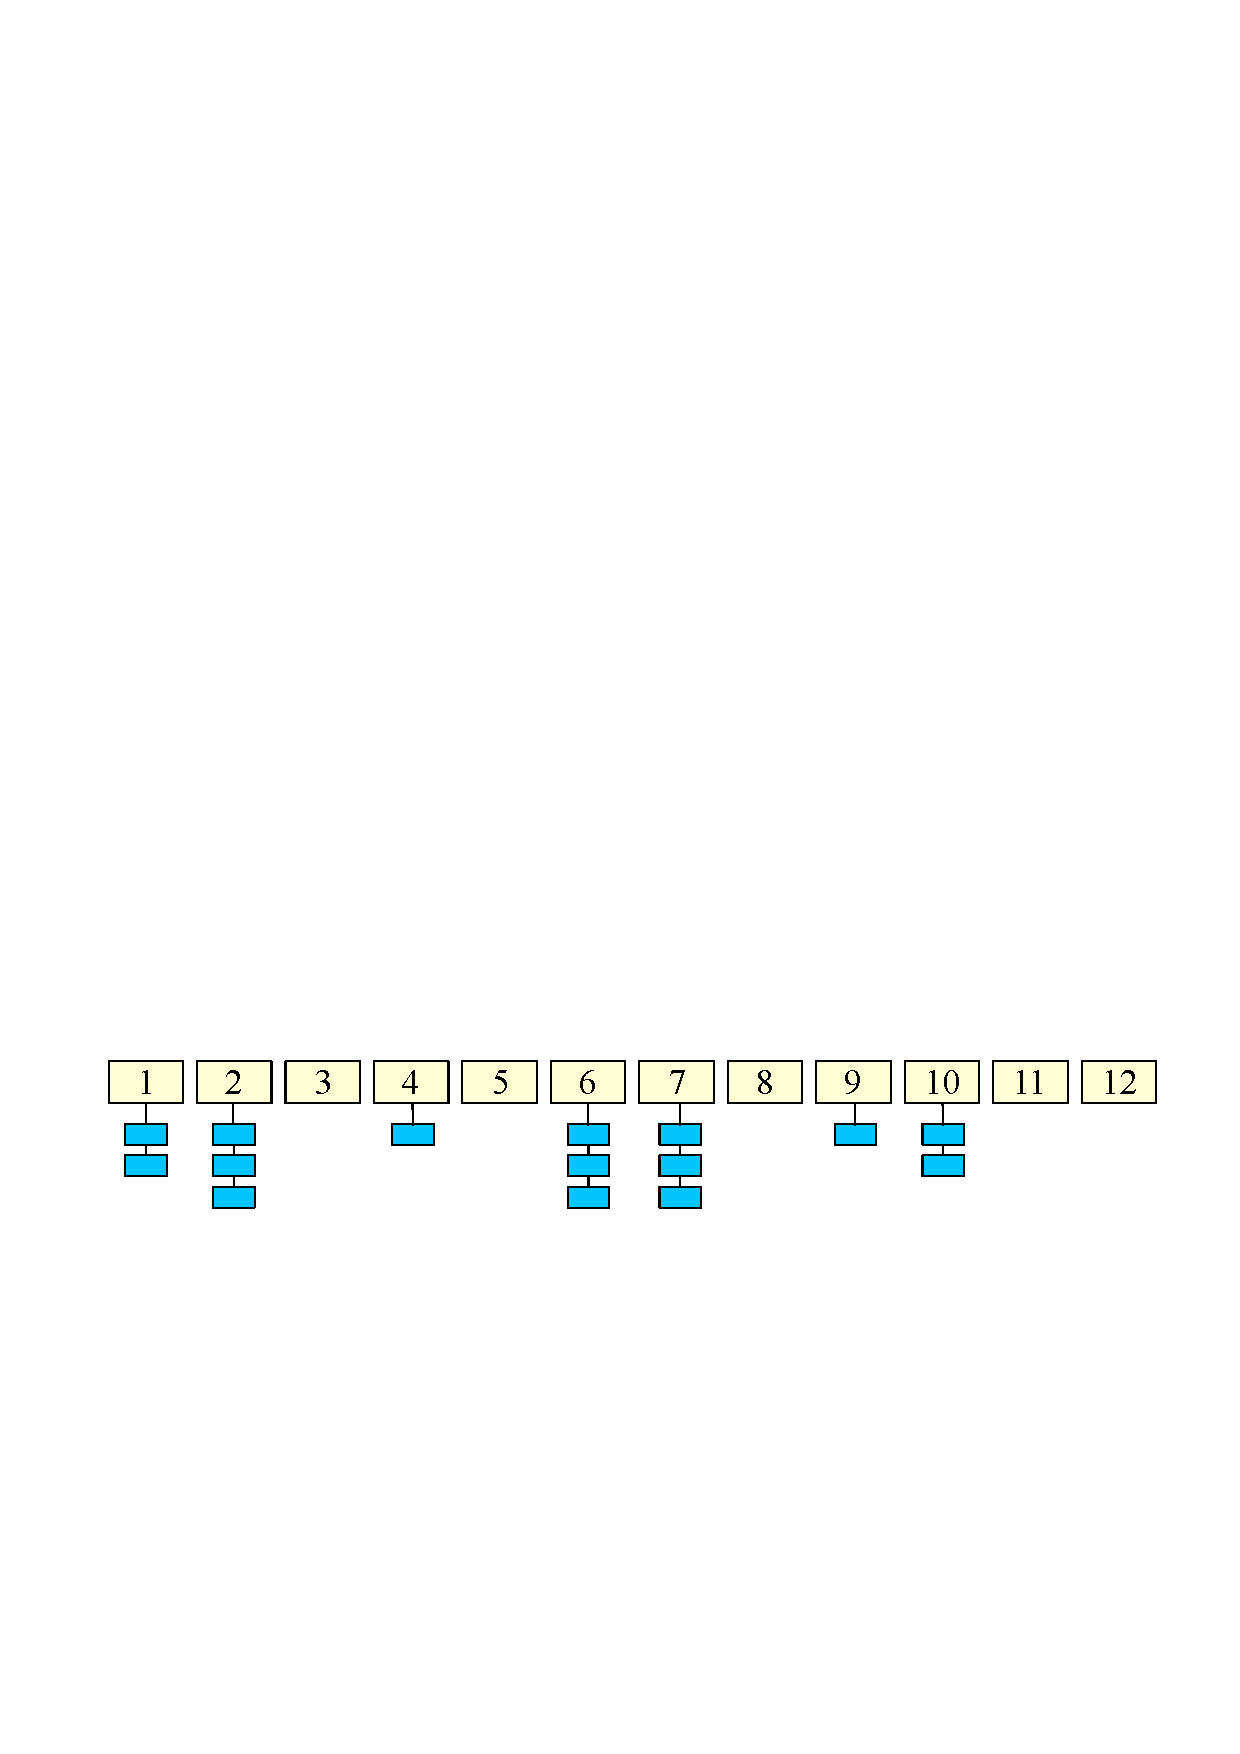
\includegraphics[width=.8\textwidth]{pigeonhole}
\end{figure}

% \begin{algorithm}[H]
%     \caption{Algoritmo di ordinamento PigeonholeSort}
%     \input{pigeonholeSort}
% \end{algorithm}

% \clearpage
\subsection{Bucket Sort}

Se i valori in input sono:
\begin{enumerate}
    \item valori reali uniformemente distribuiti nell'intervallo \([0, 1)\);
    \item oppure è possibile normalizzarli nell'intervallo \([0,1)\) in tempo lineare, in quanto sono uniformemente distribuiti, allora
\end{enumerate}
è possibile usare \bucketSort, ossia una versione di \pigeonholeSort dove utilizziamo dei concetti probabilistici (l'ipotesi di uniformità) per sapere quanti elementi ci aspettiamo che siano contenuti in ogni lista.

\paragraph{Come funziona}
Divide l'intervallo in \(n\) sottovettori di dimensione \(\nicefrac{1}{n}\), detti \foreign{bucket}, e poi distribuisce gli \(n\) numeri nei \foreign{bucket}.
% Per l'ipotesi di uniformità, il numero atteso di valori nei bucket è \(1\).
I valori così inseriti possono essere riordinati tramite \insertionSort.

La complessità attesa è di \(\Omicron(n)\), molto conveniente, ma l'ipotesi sui valori dell'input è molto stringente (ossia che siano uniformente distribuiti).

\begin{figure}[H]\centering
    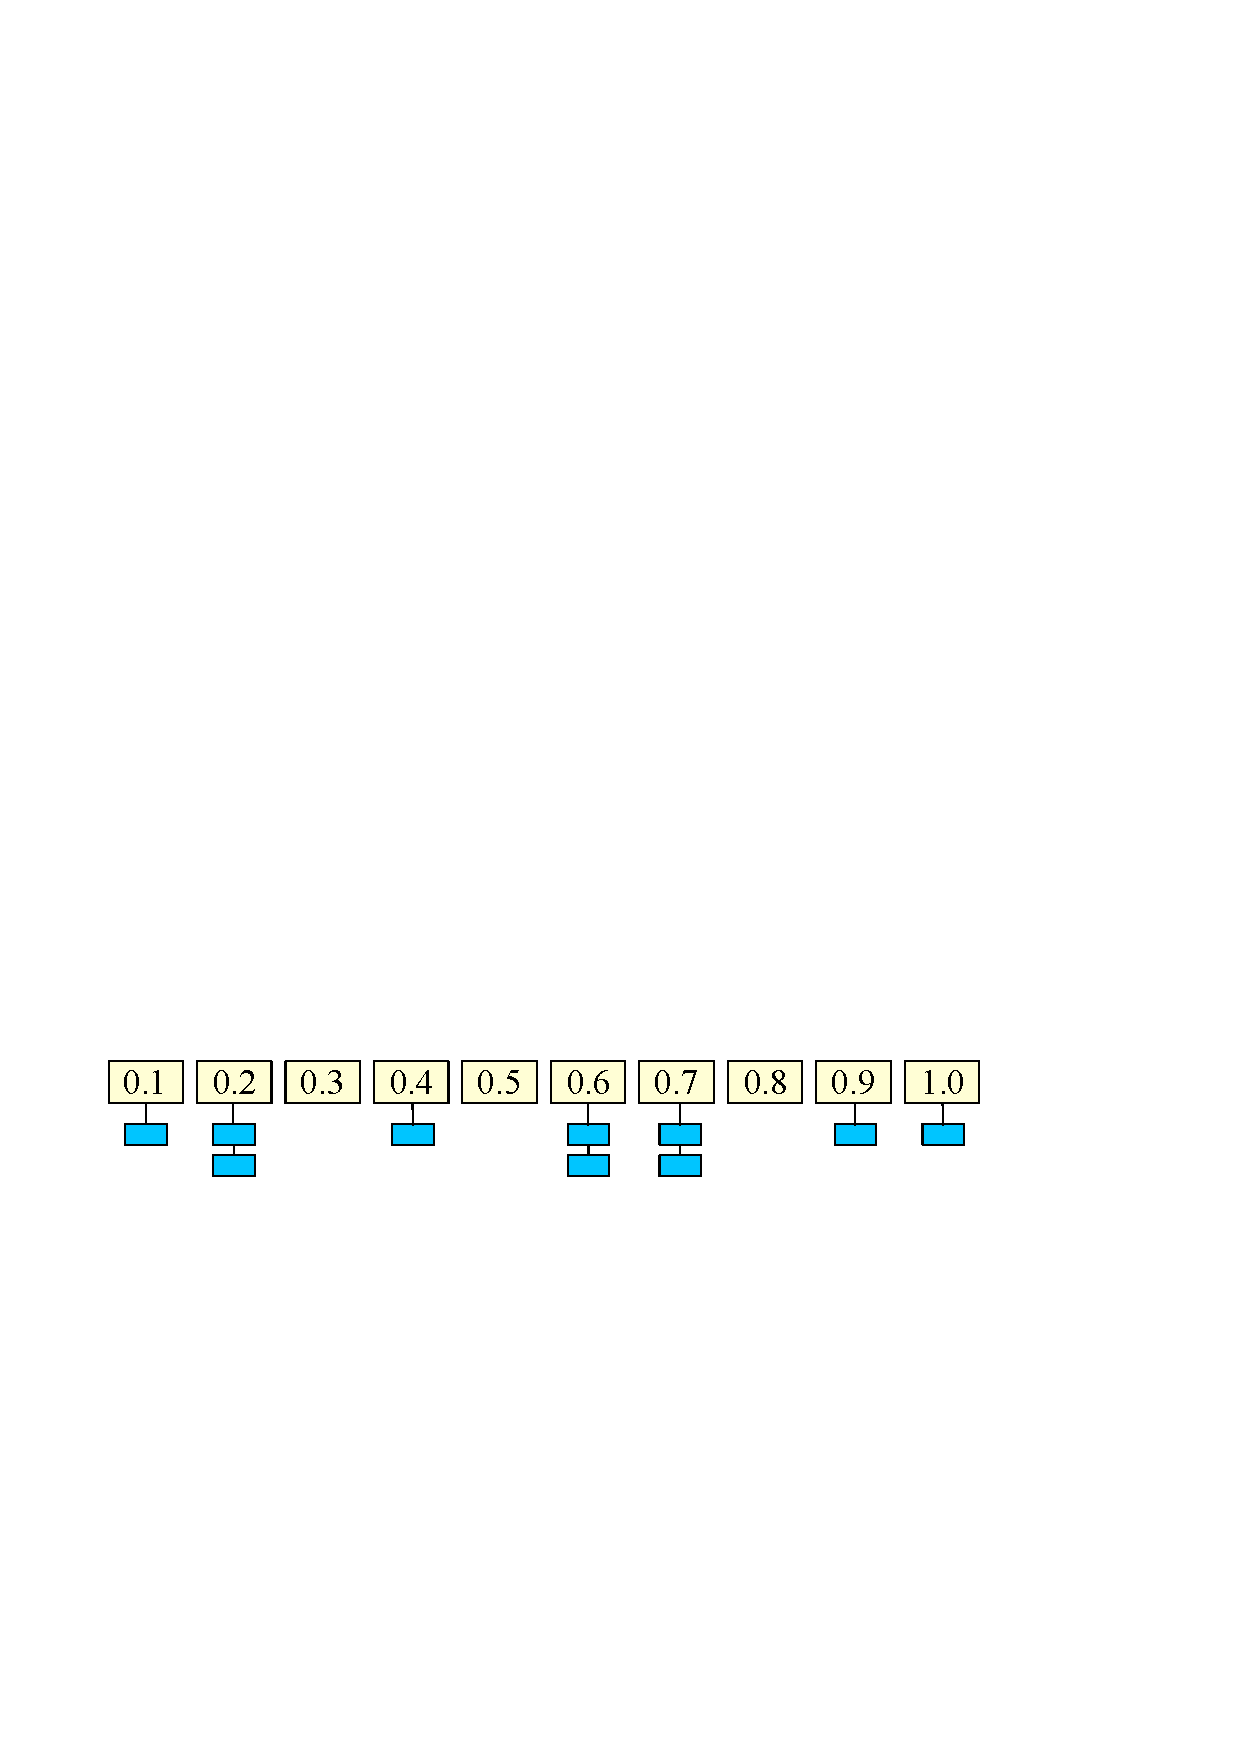
\includegraphics[width=.7\textwidth]{bucket}
    \caption[]{Il primo \foreign{bucket} conterrà gli elementi con valore contenuto nell'intervallo \([0, 0.1)\), il secondo con valori contenuti nell'intervallo \([0.1, 0.2)\) e così via. Per l'ipotesi di uniformità, il numero atteso di valori nei bucket è \(1\).}
\end{figure}

\clearpage
\subsection*{Proprietà degli algoritmi di ordinamento}

\begin{definition*}[stabilità]
Un algoritmo di ordinamento è detto \textbf{stabile} se preserva l'ordine iniziale tra due elementi con la stessa chiave.
\end{definition*}

\paragraph{Algoritmi stabili}
\insertionSort, \mergeSort, \pigeonholeSort sono algoritmi stabili, mentre \heapSort (non c'è modo di renderlo stabile) e \quickSort (esistono delle versioni complicate che lo rendono tale) non lo sono.
\`{E} possibile rendere stabile \mergeSort avendo l'accortezza di inserire ordinatamente i valori nel vettore al momento dell'unione dei sottovettori.

\begin{note}
Qualunque algoritmo di ordinamento può essere reso stabile.
Basta associare al valore da ordinare l'indice in cui si trova all'inizio dell'ordinamento.
Ordinando quindi prima per valore e poi per posizione.
% Basta usare come chiave di ordinamento la coppia (chiave, posizione iniziale).
\end{note}

\section{Rissunto algoritmi di ordinamento}

\insertionSort ha una compleesità di \(\Omega(n)\) nel caso ottimo e di \(\Omicron(n^2)\) nel caso pessimo.
\`{E} stabile, sul posto, iterativo.
Adatto per piccoli valori (non utilizzare \quickSort) e sequenze quasi ordinate.

\mergeSort ha una complessità di \(\Theta(n \log n)\), è stabile ma richiede \(\Omicron(n)\) spazio aggiuntivo, è ricorsivo (richiede \(\Omicron(\log n)\) spazio nello \foreign{stack}).
Buona performance in \foreign{cache}, buona parallelizzazione.

\heapSort ha una complessità di \(\Theta(n \log n)\), non stabile, sul posto, iterativo.
Cattiva performance in cache, cattiva parallelizzazione viene quindi preferito in sistemi embedded dove parallelizzazione e memoria aggiuntiva non vengono considerati.

\quickSort \(\Omicron(n \log n)\) in media, \(\Omicron(n^2)\) nel caso peggiore, non stabile, ricorsivo (richiede \(\Omicron(\log n)\) spazio nello \foreign{stack}).
Buona performance in cache, buona parallelizzazione, buoni fattori moltiplicativi.
\`{E} una delle scelte migliori grazie al meccanismo di randomizzazione permette nel caso medio di avere una complessità di \(n \log n\).

\countingSort \(\Theta(n+k)\), richiede \(\Omicron(k)\) memoria aggiuntiva, iterativo.
Molto veloce quando \(k = \Omicron(n)\).

\pigeonholeSort \(\Theta(n+k)\), stabile, richiede \(\Omicron(n+k)\) memoria aggiuntiva, iterativo.
Molto veloce quando \(k = \Omicron(n)\).

\countingSort e \pigeonholeSort vengono utilizzati quando sappiamo qualcosa sui dati in input.

\bucketSort \(\Omicron(n)\) nel caso i valori siano distribuiti uniformemente, stabile, richiede \(\Omicron(n)\) spazio aggiuntivo.

\shellSort \(\Omicron(n \sqrt{n})\), stabile, adatto per piccoli valori, sequenze quasi ordinate.
\`{E} una versione migliorata di \insertionSort.

\ifsubfile
\end{document}
\fi
